\documentclass[11pt,a4paper]{article}
\usepackage[margin=2.3cm]{geometry}
\usepackage{booktabs,longtable,array,graphicx,amsmath,amssymb,multirow,float}
\usepackage{caption}
\captionsetup{font=small,labelfont=bf,skip=4pt}
\usepackage[hidelinks]{hyperref}
\usepackage{enumitem}
\setlist[itemize]{leftmargin=1.4em,itemsep=2pt,topsep=3pt}
\renewcommand{\arraystretch}{1.05}
\sloppy

\begin{document}

\begin{center}
{\Large\bfseries Supplementary Information}\\[6pt]
{\large Semantic-Guided Differentiable Hierarchical Temporal Graph Learning\\
for Class-Imbalanced Log Anomaly Detection}\\[8pt]
Caizhong Que$^{1,2}$, Guofang Dong$^{1,2,*}$\\[4pt]
{\small $^1$ School of Electrical and Information Engineering, Yunnan Minzu University,
Kunming 650504, China\\
$^2$ Key Laboratory of Unmanned Autonomous Systems of Yunnan Province,
Yunnan Minzu University, Kunming 650504, China\\
$^*$ Corresponding author: dongguofangyx@163.com}
\end{center}

\vspace{-4pt}
\hrule
\vspace{6pt}

\noindent This file contains 13 supplementary tables, two supplementary figures, two
short supplementary texts and the reference list for the literature values quoted in
Supplementary Table S10. Per-seed metrics for all 724 training runs are provided in the
separate workbook \emph{Source Data 1}; the code that produced every item is available
in the accompanying repository.

\begin{itemize}
\item S1 Statistical testing protocol
\item S2 Additional metrics for the main comparison
\item S3 Seed-level results for imbalance learning and prototype configurations
\item S4 Final hyper-parameters and implementation settings
\item S5 Hyper-parameter sensitivity analysis
\item S6 Semantic and entity shortcut ablations
\item S7 Robustness to parsing noise
\item S8 Entity identifiability and entity holdout
\item S9 Masked-template pretraining baseline
\item S10 Literature reference values and protocol differences
\item S11 Baseline taxonomy and comparison protocol
\item S12 Negative-sampling strategies for contrastive pretraining
\item S13 Semantic field sources and leakage controls
\item Supplementary Figures S1--S2
\item Supplementary Text S1 Experimental design and reproducibility protocol
\item Supplementary Text S2 Data provenance and file hashes
\end{itemize}

\clearpage
\subsection*{Supplementary Text S1. Experimental design and reproducibility protocol}

\noindent\textbf{Data and leakage control.} Every dataset is parsed with Drain
(depth 4, similarity 0.5) fitted on training-split events only and then frozen;
validation and test templates that were not seen in training map to a placeholder. The
semantic dictionaries for action and state are fixed before any label is inspected, and
no test-set template, anomaly label, large language model or external anomaly knowledge
base contributes to them. Where a dataset has an official session key (HDFS block,
OpenStack instance, SSH derived key) that key defines the outer sample; otherwise an
adaptive idle-gap threshold, estimated from the training partition alone, is used.
Splits are 60/20/20; BGL and Thunderbird use a session-stratified random split with a
fixed seed, HDFS and OpenStack use a time-ordered split (HDFS groups sessions that share
a raw event to prevent replication leakage), and a time-ordered BGL cache is kept for
the template-evolution stress test.

\noindent\textbf{Model selection and statistics.} Five seeds (42, 123, 256, 512,
1024) are used for the principal experiments. Models are selected on validation AUPRC
with early stopping (patience 10) and the decision threshold is calibrated on the
validation split by maximising F1; the test split is never used for selection.
Comparative claims are supported by paired Wilcoxon signed-rank tests on matched seeds
with Holm correction inside each comparison family, reported together with Cliff's
$\delta$; because five paired seeds give a smallest attainable two-sided $p$ of 0.0625,
the paper interprets effect sizes and cross-dataset consistency rather than a binary
significance threshold (Supplementary Table S1).

\noindent\textbf{Reproducibility.} Each run writes a manifest with the SHA-256
hashes of the raw data, the processed cache and the configuration files, together with
the seed and the effective model configuration; checkpoints store the optimiser state
and the random-number-generator state. The scripts that produce every table and figure
are listed in the repository, and the exact package versions are pinned.

\clearpage
\subsection*{Supplementary Text S2. Data provenance and file hashes}

\noindent Processed caches used for the controlled experiments:

\begin{center}
\begin{tabular}{llll}
\toprule
Dataset & Cache built (UTC) & Code revision & sessions.parquet SHA-256 \\
\midrule
bgl & 2026-08-29T12:14:17 & \texttt{a35db7ff0c} & \texttt{2a9cb2589291bed7\ldots} \\
hdfs & 2026-08-29T11:32:16 & \texttt{a35db7ff0c} & \texttt{439dc81b2e177bed\ldots} \\
openstack & 2026-08-29T11:05:47 & \texttt{a35db7ff0c} & \texttt{59c7834426ff7176\ldots} \\
ssh & 2026-08-29T11:06:54 & \texttt{a35db7ff0c} & \texttt{aa09e7268eadf0a1\ldots} \\
thunderbird & 2026-08-29T12:35:04 & \texttt{a35db7ff0c} & \texttt{f246c7d2dfd46d68\ldots} \\
\bottomrule
\end{tabular}
\end{center}

\noindent The full hashes, the raw-file hashes and the per-run manifests are included
in the repository under \texttt{data/processed/*/manifest.json} and
\texttt{outputs/*/main/**/training\_manifest.json}.

\clearpage
\begin{table}[H]
\centering
\caption*{\textbf{Supplementary Table S1.} Paired statistical comparisons. Wilcoxon signed-rank tests use the same random seed as the pairing unit; $q_{\mathrm{Holm}}$ values are corrected within each family and metric, and Cliff's $\delta$ is the effect size (positive = the first method is better). With five paired seeds the smallest attainable two-sided $p$ is 0.0625.}
{\small
\resizebox{\textwidth}{!}{%
\begin{tabular}{llccrrrrl}
\toprule
Dataset & Comparison & Metric & Pairs & $\Delta$ (pt) & $p$ & $q_{\mathrm{Holm}}$ & Cliff's $\delta$ & Direction \\
\midrule
\multicolumn{4}{l}{\textit{primary}} &  &  &  &  &  \\
ssh & GRU-flat (L0) & F1 & 5 & +0.50 & 1.0000 & 1.0000 & -0.04 & $-$ \\
ssh & GRU-flat (L0) & AUPRC & 5 & +0.69 & 0.3125 & 0.6250 & +0.28 & $+$ \\
hdfs & TCN & F1 & 5 & +4.02 & 0.0625 & 0.3125 & +1.00 & $+$ \\
hdfs & Transformer & AUPRC & 5 & -0.22 & 0.0625 & 0.3125 & -1.00 & $-$ \\
bgl & GNN-flat & F1 & 5 & +0.02 & 0.3125 & 0.9375 & +0.36 & $+$ \\
bgl & GNN-flat & AUPRC & 5 & -0.00 & 0.1875 & 0.5625 & -0.44 & $-$ \\
openstack & GRU-flat (L0) & F1 & 5 & -0.00 & 1.0000 & 1.0000 & -0.12 & $-$ \\
openstack & GRU-flat (L0) & AUPRC & 5 & -0.00 & 1.0000 & 1.0000 & -0.04 & $-$ \\
thunderbird & GNN-flat & F1 & 5 & -0.30 & 0.0625 & 0.3125 & -1.00 & $-$ \\
thunderbird & GNN-flat & AUPRC & 5 & -0.09 & 0.1250 & 0.5000 & -0.68 & $-$ \\
\multicolumn{4}{l}{\textit{vs GRU-flat (L0)}} &  &  &  &  &  \\
ssh & GRU-flat (L0) & F1 & 5 & +0.50 & 1.0000 & 1.0000 & -0.04 & $-$ \\
ssh & GRU-flat (L0) & AUPRC & 5 & +0.69 & 0.3125 & 1.0000 & +0.28 & $+$ \\
hdfs & GRU-flat (L0) & F1 & 5 & +5.41 & 0.0625 & 0.3125 & +1.00 & $+$ \\
hdfs & GRU-flat (L0) & AUPRC & 5 & -0.10 & 0.4375 & 1.0000 & -0.52 & $-$ \\
bgl & GRU-flat (L0) & F1 & 5 & +0.06 & 0.1875 & 0.7500 & +0.76 & $+$ \\
bgl & GRU-flat (L0) & AUPRC & 5 & +0.00 & 0.4375 & 1.0000 & +0.44 & $+$ \\
openstack & GRU-flat (L0) & F1 & 5 & -0.00 & 1.0000 & 1.0000 & -0.12 & $-$ \\
openstack & GRU-flat (L0) & AUPRC & 5 & -0.00 & 1.0000 & 1.0000 & -0.04 & $-$ \\
thunderbird & GRU-flat (L0) & F1 & 5 & -0.00 & 1.0000 & 1.0000 & +0.08 & $+$ \\
thunderbird & GRU-flat (L0) & AUPRC & 5 & +0.05 & 0.3125 & 1.0000 & +0.28 & $+$ \\
\multicolumn{4}{l}{\textit{module step}} &  &  &  &  &  \\
hdfs & 多正常原型 L7 vs L6 & F1 & 5 & +9.89 & 0.0625 & 0.3750 & +1.00 & $+$ \\
hdfs & 完整模型 L7 vs L0 & F1 & 5 & +5.41 & 0.0625 & 0.3750 & +1.00 & $+$ \\
hdfs & 原型多样/均衡 L7b vs L7 & F1 & 5 & -0.86 & 0.1875 & 0.5625 & -0.28 & $-$ \\
ssh & 多正常原型 L7 vs L6 & F1 & 5 & +1.39 & 0.0625 & 0.3750 & +0.36 & $+$ \\
ssh & 完整模型 L7 vs L0 & F1 & 5 & +0.50 & 1.0000 & 1.0000 & -0.04 & $-$ \\
ssh & 原型多样/均衡 L7b vs L7 & F1 & 5 & -1.47 & 0.2500 & 0.5625 & -0.40 & $-$ \\
\bottomrule
\end{tabular}
}
}
\end{table}

\begin{table}[H]
\centering
\caption*{\textbf{Supplementary Table S2.} Additional metrics for the main comparison (mean $\pm$ standard deviation over the five matched random seeds). MCC and balanced accuracy are computed from the reported precision, recall and the test-set class composition.}
{\scriptsize
\resizebox{\textwidth}{!}{%
\begin{tabular}{llcrrrrrrr}
\toprule
Dataset & Method & Seeds & AUPRC & AUROC & Precision & Recall & F1 & MCC & Balanced accuracy \\
\midrule
bgl & TCN & 5 & 1.0000 $\pm$ 0.0000 & 1.0000 $\pm$ 0.0000 & 0.9979 $\pm$ 0.0015 & 0.9989 $\pm$ 0.0009 & 0.9984 $\pm$ 0.0009 & 0.9981 $\pm$ 0.0010 & 0.9992 $\pm$ 0.0005 \\
bgl & Transformer & 5 & 1.0000 $\pm$ 0.0000 & 1.0000 $\pm$ 0.0000 & 0.9975 $\pm$ 0.0015 & 0.9994 $\pm$ 0.0004 & 0.9985 $\pm$ 0.0008 & 0.9981 $\pm$ 0.0010 & 0.9994 $\pm$ 0.0003 \\
bgl & GNN-flat & 5 & 1.0000 $\pm$ 0.0000 & 1.0000 $\pm$ 0.0000 & 0.9980 $\pm$ 0.0008 & 0.9991 $\pm$ 0.0004 & 0.9986 $\pm$ 0.0003 & 0.9983 $\pm$ 0.0004 & 0.9993 $\pm$ 0.0002 \\
bgl & GRU-flat (L0) & 5 & 1.0000 $\pm$ 0.0000 & 1.0000 $\pm$ 0.0000 & 0.9980 $\pm$ 0.0005 & 0.9983 $\pm$ 0.0007 & 0.9981 $\pm$ 0.0006 & 0.9978 $\pm$ 0.0007 & 0.9989 $\pm$ 0.0004 \\
bgl & SDHTG (L7) & 5 & 1.0000 $\pm$ 0.0000 & 1.0000 $\pm$ 0.0000 & 0.9979 $\pm$ 0.0010 & 0.9996 $\pm$ 0.0003 & 0.9987 $\pm$ 0.0004 & 0.9985 $\pm$ 0.0005 & 0.9996 $\pm$ 0.0001 \\
hdfs & TCN & 5 & 0.9988 $\pm$ 0.0009 & 1.0000 $\pm$ 0.0000 & 0.9113 $\pm$ 0.0231 & 0.9989 $\pm$ 0.0011 & 0.9530 $\pm$ 0.0124 & 0.9533 $\pm$ 0.0121 & 0.9987 $\pm$ 0.0005 \\
hdfs & Transformer & 5 & 0.9996 $\pm$ 0.0002 & 1.0000 $\pm$ 0.0000 & 0.9069 $\pm$ 0.0608 & 0.9874 $\pm$ 0.0243 & 0.9439 $\pm$ 0.0228 & 0.9447 $\pm$ 0.0220 & 0.9929 $\pm$ 0.0117 \\
hdfs & GNN-flat & 5 & 0.9867 $\pm$ 0.0176 & 0.9998 $\pm$ 0.0003 & 0.8295 $\pm$ 0.0642 & 0.9996 $\pm$ 0.0008 & 0.9056 $\pm$ 0.0375 & 0.9087 $\pm$ 0.0352 & 0.9983 $\pm$ 0.0005 \\
hdfs & GRU-flat (L0) & 5 & 0.9984 $\pm$ 0.0016 & 1.0000 $\pm$ 0.0000 & 0.8867 $\pm$ 0.0430 & 0.9990 $\pm$ 0.0014 & 0.9391 $\pm$ 0.0234 & 0.9401 $\pm$ 0.0225 & 0.9986 $\pm$ 0.0005 \\
hdfs & SDHTG (L7) & 5 & 0.9974 $\pm$ 0.0019 & 0.9997 $\pm$ 0.0006 & 0.9955 $\pm$ 0.0046 & 0.9910 $\pm$ 0.0040 & 0.9932 $\pm$ 0.0023 & 0.9931 $\pm$ 0.0023 & 0.9954 $\pm$ 0.0020 \\
openstack & TCN & 5 & 0.9998 $\pm$ 0.0000 & 0.9997 $\pm$ 0.0000 & 0.9991 $\pm$ 0.0020 & 0.9930 $\pm$ 0.0024 & 0.9960 $\pm$ 0.0010 & 0.9913 $\pm$ 0.0022 & 0.9960 $\pm$ 0.0010 \\
openstack & Transformer & 5 & 0.9999 $\pm$ 0.0001 & 0.9999 $\pm$ 0.0001 & 0.9956 $\pm$ 0.0044 & 0.9974 $\pm$ 0.0024 & 0.9965 $\pm$ 0.0025 & 0.9923 $\pm$ 0.0055 & 0.9960 $\pm$ 0.0029 \\
openstack & GNN-flat & 5 & 0.9999 $\pm$ 0.0001 & 0.9999 $\pm$ 0.0001 & 0.9905 $\pm$ 0.0064 & 0.9982 $\pm$ 0.0039 & 0.9943 $\pm$ 0.0019 & 0.9875 $\pm$ 0.0043 & 0.9933 $\pm$ 0.0025 \\
openstack & GRU-flat (L0) & 5 & 1.0000 $\pm$ 0.0000 & 1.0000 $\pm$ 0.0000 & 0.9983 $\pm$ 0.0039 & 1.0000 $\pm$ 0.0000 & 0.9991 $\pm$ 0.0020 & 0.9981 $\pm$ 0.0043 & 0.9989 $\pm$ 0.0024 \\
openstack & SDHTG (L7) & 5 & 1.0000 $\pm$ 0.0001 & 1.0000 $\pm$ 0.0001 & 0.9991 $\pm$ 0.0020 & 0.9991 $\pm$ 0.0020 & 0.9991 $\pm$ 0.0012 & 0.9981 $\pm$ 0.0026 & 0.9990 $\pm$ 0.0013 \\
ssh & TCN & 5 & 0.9729 $\pm$ 0.0272 & 0.9971 $\pm$ 0.0019 & 0.8781 $\pm$ 0.0251 & 0.9944 $\pm$ 0.0124 & 0.9324 $\pm$ 0.0130 & 0.9234 $\pm$ 0.0143 & 0.9861 $\pm$ 0.0055 \\
ssh & Transformer & 5 & 0.7484 $\pm$ 0.0905 & 0.9283 $\pm$ 0.0291 & 0.7966 $\pm$ 0.0715 & 0.7000 $\pm$ 0.2689 & 0.7132 $\pm$ 0.2068 & 0.6960 $\pm$ 0.1788 & 0.8348 $\pm$ 0.1280 \\
ssh & GNN-flat & 5 & 0.4171 $\pm$ 0.0609 & 0.8356 $\pm$ 0.0229 & 0.5052 $\pm$ 0.0445 & 0.6444 $\pm$ 0.0795 & 0.5651 $\pm$ 0.0500 & 0.4913 $\pm$ 0.0598 & 0.7713 $\pm$ 0.0382 \\
ssh & GRU-flat (L0) & 5 & 0.9854 $\pm$ 0.0122 & 0.9920 $\pm$ 0.0111 & 0.9766 $\pm$ 0.0131 & 0.9278 $\pm$ 0.0248 & 0.9515 $\pm$ 0.0168 & 0.9444 $\pm$ 0.0190 & 0.9621 $\pm$ 0.0128 \\
ssh & SDHTG (L7) & 5 & 0.9922 $\pm$ 0.0031 & 0.9985 $\pm$ 0.0006 & 0.9943 $\pm$ 0.0128 & 0.9222 $\pm$ 0.0362 & 0.9565 $\pm$ 0.0183 & 0.9510 $\pm$ 0.0201 & 0.9607 $\pm$ 0.0178 \\
thunderbird & TCN & 5 & 0.9996 $\pm$ 0.0001 & 1.0000 $\pm$ 0.0000 & 0.9997 $\pm$ 0.0004 & 0.9943 $\pm$ 0.0017 & 0.9970 $\pm$ 0.0007 & 0.9970 $\pm$ 0.0007 & 0.9971 $\pm$ 0.0008 \\
thunderbird & Transformer & 5 & 0.9994 $\pm$ 0.0006 & 0.9999 $\pm$ 0.0003 & 0.9988 $\pm$ 0.0026 & 0.9960 $\pm$ 0.0022 & 0.9974 $\pm$ 0.0023 & 0.9974 $\pm$ 0.0023 & 0.9980 $\pm$ 0.0011 \\
thunderbird & GNN-flat & 5 & 0.9998 $\pm$ 0.0001 & 1.0000 $\pm$ 0.0000 & 1.0000 $\pm$ 0.0000 & 0.9978 $\pm$ 0.0006 & 0.9989 $\pm$ 0.0003 & 0.9989 $\pm$ 0.0003 & 0.9989 $\pm$ 0.0003 \\
thunderbird & GRU-flat (L0) & 5 & 0.9983 $\pm$ 0.0001 & 0.9996 $\pm$ 0.0004 & 0.9996 $\pm$ 0.0006 & 0.9922 $\pm$ 0.0009 & 0.9959 $\pm$ 0.0005 & 0.9959 $\pm$ 0.0005 & 0.9961 $\pm$ 0.0005 \\
thunderbird & SDHTG (L7) & 5 & 0.9989 $\pm$ 0.0008 & 0.9996 $\pm$ 0.0005 & 0.9997 $\pm$ 0.0004 & 0.9921 $\pm$ 0.0012 & 0.9959 $\pm$ 0.0006 & 0.9959 $\pm$ 0.0006 & 0.9960 $\pm$ 0.0006 \\
\bottomrule
\end{tabular}
}
}
\end{table}

\begin{table}[H]
\centering
\caption*{\textbf{Supplementary Table S3.} Imbalance-learning and prototype configurations on SSH. Each configuration is trained with the same protocol as the main experiments (30 epochs, three seeds); the corresponding cross-dataset incremental ladder is reported in the main text.}
{\small
\begin{tabular}{lcrr}
\toprule
Configuration & Seeds & AUPRC & F1 \\
\midrule
bce & 3 & 0.9720 $\pm$ 0.0156 & 0.9328 $\pm$ 0.0371 \\
focal & 3 & 0.9874 $\pm$ 0.0154 & 0.9612 $\pm$ 0.0428 \\
multi\_prototype & 3 & 0.9939 $\pm$ 0.0024 & 0.9508 $\pm$ 0.0314 \\
multi\_prototype\_div & 3 & 0.9932 $\pm$ 0.0025 & 0.9664 $\pm$ 0.0229 \\
no\_prototype & 3 & 0.9882 $\pm$ 0.0055 & 0.9372 $\pm$ 0.0084 \\
single\_prototype & 3 & 0.9931 $\pm$ 0.0031 & 0.9508 $\pm$ 0.0314 \\
weighted\_bce & 3 & 0.9845 $\pm$ 0.0147 & 0.9521 $\pm$ 0.0349 \\
\bottomrule
\end{tabular}
}
\end{table}

\begin{table}[H]
\centering
\caption*{\textbf{Supplementary Table S4.} Final hyper-parameters and implementation settings, with the configuration key that carries each value. Parameters without a sensitivity scan are fixed at the stated value.}
{\scriptsize
\resizebox{\textwidth}{!}{%
\begin{tabular}{p{1.2cm}p{3.4cm}p{2.6cm}p{3.4cm}p{4.2cm}}
\toprule
Symbol & Meaning & Final value & Sensitivity scan & Verified against \\
\midrule
K & number of normal prototypes & 8 & 1, 2, 4, 16 & configs/model/sdhtg.yaml: num\_normal\_prototypes \\
tau\_p & prototype soft-assignment temperature & 0.10 & 0.05, 0.20, 0.50 & configs/model/sdhtg.yaml: prototype\_temperature; sens\_prototype\_temperature\_* \\
lambda\_p & prototype-distance scale & learned (softplus) & fixed at 0, 0.25, 0.5, 1.0, 2.0 & prototype\_scale\_override defaults to null; sens\_prototype\_scale\_* \\
m & prototype margin & 0.5 & not scanned (code default family) & configs/experiment/*.yaml: loss.prototype\_margin \\
rho\_p & prototype similarity threshold & 0.20 (code default) & not scanned & src/sdhtg/models/config.py default \\
tau\_b & boundary temperature (annealed 1.0 -> value) & 0.10 & final value 0.05, 0.25, 0.50, 1.00 & configs/model/sdhtg.yaml: boundary.final\_temperature \\
(r\_A, r\_E) & target action / entity boundary rates & 0.05 / 0.01 & 0.01/0.005, 0.01/0.001, 0.10/0.02, 0.10/0.05 & configs/experiment/*.yaml: loss.*\_boundary\_rate \\
R\_l & local temporal radius (status/action/entity) & 8 / 4 / 2 & halved (4/2/1), doubled (16/8/4) & configs/model/sdhtg.yaml: local\_temporal\_radius \\
K\_l & same-semantic neighbours (status/action/entity) & 4 / 4 / 2 & halved (2/2/1), doubled (8/8/4) & configs/model/sdhtg.yaml: semantic\_neighbors \\
eps\_m & membership-edge threshold & 1e-6 & 1e-8, 1e-4, 1e-2 & configs/model/sdhtg.yaml: hierarchy.membership\_epsilon \\
gamma & focal modulation exponent & 2.0 & not scanned & configs/experiment/*.yaml: loss.focal\_gamma \\
beta & effective-number weighting exponent & 0.9999 & not scanned & configs/experiment/*.yaml: loss.effective\_number\_beta \\
w\_proto / w\_div / w\_bal & prototype, diversity, balance loss weights & 0.05 / 0.1 / 0.1 & diversity+balance removed in the final model & configs/experiment/*.yaml: loss.prototype\_*\_weight \\
-- & masked-template pretraining (LogBERT route, supplementary baseline) & 15\% mask, 10 epochs & not scanned & scripts/train\_mlm\_baseline.py \\
\bottomrule
\end{tabular}
}
}
\end{table}

\begin{table}[H]
\centering
\caption*{\textbf{Supplementary Table S5.} Hyper-parameter sensitivity scan on SSH. Each variant is trained under the default configuration with one parameter changed; the reference is the default configuration evaluated on the same seeds (validation AUPRC 0.9853, test AUPRC 0.9941, test F1 0.9561). Per-seed values are provided in Source Data 1.}
{\scriptsize
\resizebox{\textwidth}{!}{%
\begin{tabular}{lcrrrr}
\toprule
Setting (group\_variant) & Seeds & Validation AUPRC & Test AUPRC & Test F1 & $\Delta$F1 vs default (pt) \\
\midrule
boundary\textbackslash{}\_rate\textbackslash{}\_ra001\textbackslash{}\_re0001 & 3 & 0.9857 & 0.9935 & 0.9664 & +1.03 \\
boundary\textbackslash{}\_rate\textbackslash{}\_ra001\textbackslash{}\_re0005 & 3 & 0.9816 & 0.9960 & 0.9710 & +1.49 \\
boundary\textbackslash{}\_rate\textbackslash{}\_ra010\textbackslash{}\_re0020 & 3 & 0.9850 & 0.9941 & 0.9515 & -0.46 \\
boundary\textbackslash{}\_rate\textbackslash{}\_ra010\textbackslash{}\_re0050 & 3 & 0.9853 & 0.9934 & 0.9515 & -0.46 \\
boundary\textbackslash{}\_temperature\textbackslash{}\_tau005 & 3 & 0.9858 & 0.9938 & 0.9521 & -0.40 \\
boundary\textbackslash{}\_temperature\textbackslash{}\_tau025 & 3 & 0.9858 & 0.9930 & 0.9619 & +0.58 \\
boundary\textbackslash{}\_temperature\textbackslash{}\_tau050 & 3 & 0.9865 & 0.9941 & 0.9561 & -0.00 \\
boundary\textbackslash{}\_temperature\textbackslash{}\_tau100 & 3 & 0.9853 & 0.9934 & 0.9470 & -0.91 \\
membership\textbackslash{}\_epsilon\textbackslash{}\_eps1e-4 & 3 & 0.9856 & 0.9931 & 0.9515 & -0.46 \\
membership\textbackslash{}\_epsilon\textbackslash{}\_eps1e-8 & 3 & 0.9829 & 0.9947 & 0.9664 & +1.03 \\
prototype\textbackslash{}\_scale\textbackslash{}\_lambda000 & 3 & 0.9811 & 0.9858 & 0.9521 & -0.40 \\
prototype\textbackslash{}\_scale\textbackslash{}\_lambda025 & 3 & 0.9838 & 0.9915 & 0.9475 & -0.86 \\
prototype\textbackslash{}\_scale\textbackslash{}\_lambda050 & 3 & 0.9855 & 0.9937 & 0.9572 & +0.11 \\
prototype\textbackslash{}\_scale\textbackslash{}\_lambda100 & 3 & 0.9846 & 0.9943 & 0.9622 & +0.61 \\
prototype\textbackslash{}\_scale\textbackslash{}\_lambda200 & 3 & 0.9802 & 0.9960 & 0.9814 & +2.53 \\
prototype\textbackslash{}\_temperature\textbackslash{}\_tau005 & 3 & 0.9845 & 0.9945 & 0.9616 & +0.55 \\
prototype\textbackslash{}\_temperature\textbackslash{}\_tau020 & 3 & 0.9864 & 0.9947 & 0.9515 & -0.46 \\
prototype\textbackslash{}\_temperature\textbackslash{}\_tau050 & 3 & 0.9855 & 0.9943 & 0.9612 & +0.51 \\
prototypes\textbackslash{}\_k1 & 3 & 0.9852 & 0.9926 & 0.9410 & -1.51 \\
prototypes\textbackslash{}\_k16 & 3 & 0.9856 & 0.9940 & 0.9561 & -0.00 \\
prototypes\textbackslash{}\_k2 & 3 & 0.9855 & 0.9932 & 0.9365 & -1.96 \\
prototypes\textbackslash{}\_k4 & 3 & 0.9856 & 0.9930 & 0.9514 & -0.47 \\
semantic\textbackslash{}\_neighbors\textbackslash{}\_double & 3 & 0.9824 & 0.9951 & 0.9665 & +1.04 \\
semantic\textbackslash{}\_neighbors\textbackslash{}\_half & 3 & 0.9830 & 0.9939 & 0.9566 & +0.05 \\
temporal\textbackslash{}\_radius\textbackslash{}\_double & 3 & 0.9849 & 0.9941 & 0.9508 & -0.53 \\
temporal\textbackslash{}\_radius\textbackslash{}\_half & 3 & 0.9857 & 0.9935 & 0.9417 & -1.44 \\
\bottomrule
\end{tabular}
}
}
\end{table}

\begin{table}[H]
\centering
\caption*{\textbf{Supplementary Table S6.} Semantic and entity shortcut controls on SSH: each row removes or alters one selected cue (entity embedding, boundary priors, action/state sources, entity identity) while keeping the remaining inputs unchanged. The last row repeats the full-input reference.}
{\small
\begin{tabular}{lcrr}
\toprule
Variant & Seeds & AUPRC & F1 \\
\midrule
entity\_unk & 5 & 0.9907 $\pm$ 0.0042 & 0.9479 $\pm$ 0.0249 \\
mask\_status\_words & 5 & 0.9937 $\pm$ 0.0034 & 0.9598 $\pm$ 0.0216 \\
no\_action\_prior & 5 & 0.9929 $\pm$ 0.0029 & 0.9538 $\pm$ 0.0193 \\
no\_action\_source & 5 & 0.9917 $\pm$ 0.0033 & 0.9449 $\pm$ 0.0265 \\
no\_entity\_embed & 5 & 0.9930 $\pm$ 0.0030 & 0.9541 $\pm$ 0.0162 \\
no\_entity\_prior & 5 & 0.9928 $\pm$ 0.0035 & 0.9573 $\pm$ 0.0110 \\
no\_status\_source & 5 & 0.9924 $\pm$ 0.0030 & 0.9482 $\pm$ 0.0269 \\
shuffle\_entity & 5 & 0.9919 $\pm$ 0.0046 & 0.9600 $\pm$ 0.0192 \\
template\_time\_only & 5 & 0.9922 $\pm$ 0.0048 & 0.9568 $\pm$ 0.0313 \\
full input (reference) & 5 & $0.9922 \pm 0.0031$ & $0.9565 \pm 0.0183$ \\
\bottomrule
\end{tabular}
}
\end{table}

\begin{table}[H]
\centering
\caption*{\textbf{Supplementary Table S7.} Paired evaluation under template-level parsing noise (SSH). Replacement, merge, split and UNK-injection corruptions are applied at rewrite rates of 20\% and 40\%; ``test\_only'' corrupts the test split, ``all'' corrupts training, validation and test. Model parameters and the decision threshold calibrated on the clean validation split are kept fixed, and the clean column re-evaluates the same weights on the clean test split. $\Delta$ is in percentage points.}
{\scriptsize
\resizebox{\textwidth}{!}{%
\begin{tabular}{lllcrrrrrr}
\toprule
Rate & Corruption & Protocol & Seeds & AUPRC$_{\mathrm{noisy}}$ & AUPRC$_{\mathrm{clean}}$ & $\Delta$AUPRC & F1$_{\mathrm{noisy}}$ & F1$_{\mathrm{clean}}$ & $\Delta$F1 \\
\midrule
$20\%$ & merge & all & 2 & 0.9926 & 0.9922 & +0.05 & 0.9412 & 0.9644 & -2.32 \\
$20\%$ & merge\_test & only & 2 & 0.9929 & 0.9918 & +0.11 & 0.9420 & 0.9722 & -3.02 \\
$20\%$ & replace & all & 2 & 0.9946 & 0.9940 & +0.05 & 0.9567 & 0.9650 & -0.83 \\
$20\%$ & replace\_test & only & 2 & 0.9933 & 0.9902 & +0.31 & 0.9333 & 0.9334 & -0.01 \\
$20\%$ & split & all & 2 & 0.9962 & 0.9966 & -0.04 & 0.9787 & 0.8959 & +8.27 \\
$20\%$ & split\_test & only & 2 & 0.9958 & 0.9961 & -0.03 & 0.9563 & 0.9718 & -1.55 \\
$20\%$ & unk & all & 2 & 0.9946 & 0.9943 & +0.03 & 0.9567 & 0.9650 & -0.83 \\
$20\%$ & unk\_test & only & 2 & 0.9919 & 0.9920 & -0.00 & 0.9575 & 0.9291 & +2.84 \\
$40\%$ & merge & all & 2 & 0.9941 & 0.9481 & +4.60 & 0.9488 & 0.4861 & +46.27 \\
$40\%$ & merge\_test & only & 2 & 0.9919 & 0.9905 & +0.14 & 0.9344 & 0.9499 & -1.55 \\
$40\%$ & replace & all & 2 & 0.9944 & 0.9944 & +0.00 & 0.9420 & 0.9567 & -1.47 \\
$40\%$ & replace\_test & only & 2 & 0.9949 & 0.9946 & +0.03 & 0.9567 & 0.9656 & -0.88 \\
$40\%$ & split & all & 2 & 0.9944 & 0.9940 & +0.03 & 0.9571 & 0.9646 & -0.74 \\
$40\%$ & split\_test & only & 2 & 0.9943 & 0.9953 & -0.10 & 0.9426 & 0.9567 & -1.41 \\
$40\%$ & unk & all & 2 & 0.9925 & 0.9912 & +0.13 & 0.9429 & 0.9650 & -2.21 \\
$40\%$ & unk\_test & only & 2 & 0.9932 & 0.9912 & +0.21 & 0.9644 & 0.9179 & +4.65 \\
\bottomrule
\end{tabular}
}
}
\end{table}

\begin{table}[H]
\centering
\caption*{\textbf{Supplementary Table S8.} Entity-identifiability evaluation. The entity identities covering about 20\% of the test sessions are masked to a placeholder in training, validation and test, and the model is retrained; ``seen'' and ``holdout'' then refer to the same weights and the same calibrated threshold. OpenStack has no negatives in the holdout group, so AUPRC is undefined there.}
{\small
\begin{tabular}{llcccrrrr}
\toprule
Dataset & Group & Seeds & Samples & Positives & AUPRC & F1 & Precision & Recall \\
\midrule
bgl & all & 2 & 31688 & 5280 & 1.0000 & 0.9977 & 0.9969 & 0.9986 \\
bgl & holdout & 2 & 11530 & 1580 & 1.0000 & 0.9954 & 0.9934 & 0.9975 \\
bgl & seen & 2 & 20000 & 3697 & 1.0000 & 0.9987 & 0.9984 & 0.9991 \\
openstack & all & 2 & 417 & 228 & 0.9999 & 0.8535 & 0.7734 & 1.0000 \\
openstack & holdout & 2 & 169 & 169 & -- & 1.0000 & 1.0000 & 1.0000 \\
openstack & seen & 2 & 248 & 59 & 0.9992 & 0.6922 & 0.6190 & 1.0000 \\
\bottomrule
\end{tabular}
}
\end{table}

\begin{table}[H]
\centering
\caption*{\textbf{Supplementary Table S9.} Masked-template pretraining baseline under the controlled input protocol. The baseline shares the inputs, encoder depth and width, supervised objective, early-stopping rule and threshold calibration with the flat Transformer; only the 15\% masked-template pretraining stage is added. SSH and OpenStack use five seeds, BGL one (it is saturated).}
{\small
\begin{tabular}{llcrr}
\toprule
Dataset & Method & Seeds & AUPRC & F1 \\
\midrule
bgl & SDHTG & 5 & 1.0000 $\pm$ 0.0000 & 0.9987 $\pm$ 0.0004 \\
bgl & Transformer (no pretraining) & 5 & 1.0000 $\pm$ 0.0000 & 0.9985 $\pm$ 0.0008 \\
bgl & Transformer + masked-template pretraining & 1 & 0.9999 & 0.9985 \\
openstack & SDHTG & 5 & 1.0000 $\pm$ 0.0001 & 0.9991 $\pm$ 0.0012 \\
openstack & Transformer (no pretraining) & 5 & 0.9999 $\pm$ 0.0001 & 0.9965 $\pm$ 0.0025 \\
openstack & Transformer + masked-template pretraining & 5 & 0.9994 $\pm$ 0.0013 & 0.9978 $\pm$ 0.0022 \\
ssh & SDHTG & 5 & 0.9922 $\pm$ 0.0031 & 0.9565 $\pm$ 0.0183 \\
ssh & Transformer (no pretraining) & 5 & 0.7484 $\pm$ 0.0905 & 0.7132 $\pm$ 0.2068 \\
ssh & Transformer + masked-template pretraining & 5 & 0.8953 $\pm$ 0.0245 & 0.7634 $\pm$ 0.0283 \\
\bottomrule
\end{tabular}
}
\end{table}

\begin{table}[H]
\centering
\caption*{\textbf{Supplementary Table S10.} Reference values reported by prior studies under their own protocols. Differences in preprocessing, split construction, label definition, threshold selection and evaluation protocol prevent direct numerical comparison with the controlled results of this work; the table is provided for context only.}
{\scriptsize
\resizebox{\textwidth}{!}{%
\begin{tabular}{llccccclp{4.4cm}}
\toprule
Source & Method & HDFS & BGL & Thunderbird & OpenStack & SSH & Metric & Protocol note \\
\midrule
original paper & HitAnomaly & 0.983 & 0.921 & -- & 0.862 & -- & F1 & fixed time-window sessions; original Figs. 10/16/11 \\
original paper & LogAnomaly & 0.950 & 0.960 & -- & -- & -- & F1 & sliding window of 20 blocks/sessions \\
original paper & LogBERT & 0.823 & 0.908 & 0.966 & -- & -- & F1 & native session sequences; original Table 2 \\
original paper & LAnoBERT & 0.965 & 0.875 & 0.999 & -- & -- & F1 & parser-free masked LM; predictive-probability score, original Table 3 \\
original paper & DeepCASE & 0.904 & -- & -- & -- & -- & F1 & event sequences, 80\% training data; original Appendix E \\
original paper & BASN & 0.908 & 0.912 & -- & 0.889 & 0.871 & F1 & differentiable soft-reset single-level boundaries, zero-shot; original Table 6 \\
original paper & HLogformer & -- & -- & -- & -- & -- & F1 & evaluated on CloudTrail/OKTA/Amazon Reviews, not on LogHub \\
original paper & Log2vec & -- & -- & -- & -- & -- & AUC & CERT/LANL insider-threat detection, not LogHub \\
original paper & DeepTraLog & -- & -- & -- & -- & -- & F1 & TrainTicket microservice traces (F1 0.954), different data type \\
third-party reproduction & DeepLog & 0.773 & 0.861 & 0.931 & -- & -- & F1 & same-protocol reproduction reported by the LogBERT paper \\
third-party reproduction & LogAnomaly & 0.562 & 0.741 & 0.927 & -- & -- & F1 & same source; 0.29 lower than its original protocol \\
this work (controlled protocol) & SDHTG & 0.993 & 0.999 & 0.996 & 0.999 & 0.957 & F1 & outer samples, five seeds \\
\bottomrule
\end{tabular}
}
}
\end{table}

\begin{table}[H]
\centering
\caption*{\textbf{Supplementary Table S11.} Baseline taxonomy and comparison protocol. ``Controlled'' baselines are implemented and trained in this work under identical inputs, splits, seeds and threshold selection; literature references are quoted and never merged into the controlled comparisons.}
{\scriptsize
\resizebox{\textwidth}{!}{%
\begin{tabular}{p{2.4cm}p{3.4cm}p{5.2cm}p{3.4cm}}
\toprule
Category & Representative methods & Original protocol & Role in this work \\
\midrule
classical sequence & DeepLog, LogAnomaly & session template sequences, next-event and count anomalies & literature reference \\
pretrained language model & LogBERT, LAnoBERT & masked-template prediction, normal-pattern hypersphere & literature reference \\
hierarchical & HitAnomaly, HLogformer & hierarchical Transformer over session sequences or nested log entries & literature reference \\
context construction & DeepCASE & semi-supervised event clustering, two-stage detection & literature reference \\
graph-based & Log2vec, DeepTraLog & representation learning on log graphs or call graphs & literature reference \\
boundary-aware & BASN & differentiable soft-reset boundaries, no boundary labels & literature reference (closest related work) \\
controlled baselines & GRU-flat, TCN, Transformer, GNN-flat & identical template/entity/action/state/time inputs; no learned boundary, no heterogeneous graph & implemented here (main comparison) \\
imbalance learning & BCE, weighted BCE, focal, CB-focal & same inputs and splits, classification loss / prototype setting replaced & implemented here \\
masked-template pretraining & Transformer + masked-template prediction & identical inputs and encoder, 15\% template masking before supervised tuning & implemented here (supplementary baseline) \\
\bottomrule
\end{tabular}
}
}
\end{table}

\begin{table}[H]
\centering
\caption*{\textbf{Supplementary Table S12.} Negative-sampling strategies for contrastive pretraining on SSH. ``normal\_only'' pretrains on normal sessions, ``all\_train'' also uses unlabelled anomalous sessions; the suffix names the negative-selection rule (random, hardest, semi-hard, semantically filtered, no negatives, supervised contrastive). The reference value without pretraining is AUPRC $0.9922 \pm 0.0031$.}
{\small
\begin{tabular}{lcrr}
\toprule
Protocol (sampling \_ data range) & Seeds & AUPRC & F1 \\
\midrule
all\_train\_hard & 3 & 0.9800 $\pm$ 0.0166 & 0.9333 $\pm$ 0.0083 \\
all\_train\_none & 3 & 0.9937 $\pm$ 0.0023 & 0.9460 $\pm$ 0.0234 \\
all\_train\_random & 3 & 0.9830 $\pm$ 0.0077 & 0.9331 $\pm$ 0.0100 \\
all\_train\_semantic & 3 & 0.9939 $\pm$ 0.0026 & 0.9561 $\pm$ 0.0258 \\
all\_train\_semi\_hard & 3 & 0.9907 $\pm$ 0.0051 & 0.9493 $\pm$ 0.0083 \\
all\_train\_supervised & 3 & 0.9912 $\pm$ 0.0034 & 0.9365 $\pm$ 0.0174 \\
normal\_only\_hard & 3 & 0.9789 $\pm$ 0.0134 & 0.9427 $\pm$ 0.0151 \\
normal\_only\_none & 3 & 0.9918 $\pm$ 0.0055 & 0.9564 $\pm$ 0.0151 \\
normal\_only\_random & 3 & 0.9765 $\pm$ 0.0117 & 0.9378 $\pm$ 0.0088 \\
normal\_only\_semantic & 3 & 0.9950 $\pm$ 0.0024 & 0.9612 $\pm$ 0.0428 \\
normal\_only\_semi\_hard & 3 & 0.9887 $\pm$ 0.0017 & 0.9217 $\pm$ 0.0064 \\
normal\_only\_supervised & 3 & 0.9946 $\pm$ 0.0018 & 0.9566 $\pm$ 0.0254 \\
\bottomrule
\end{tabular}
}
\end{table}

\begin{table}[H]
\centering
\caption*{\textbf{Supplementary Table S13.} Sources of the semantic fields and the controls used to prevent label or test-set leakage. No field is derived from anomaly labels, test-split templates, large language models or external anomaly knowledge bases; unknown values map to placeholders.}
{\footnotesize
\resizebox{\textwidth}{!}{%
\begin{tabular}{p{1.8cm}p{4.6cm}p{4.4cm}p{4.6cm}}
\toprule
Field & Construction & Source of the labels & Leakage control \\
\midrule
template & Drain parser (depth 4, similarity 0.5) & fitted on training-split events only, then frozen & test/validation templates unseen in training map to UNK\_TEMPLATE \\
action & deterministic prior dictionary over training template texts & fixed before seeing any labels & no test-set templates, no LLM, no external anomaly knowledge \\
state & deterministic status dictionary plus template-identity fallback & fixed before seeing any labels & explicit anomaly words (failed/error/timeout) are ablated in Section 6.4 \\
entity & dataset-specific key (node, block id, host, service) & taken from the raw log fields & train-side vocabulary; unseen entities map to a placeholder \\
time & per-event inter-arrival gap, continuous-time encoding & derived from the timestamps within an outer sample & no cross-split statistics are used \\
adaptive idle threshold & median inter-event gap per entity x 2 (capped 3600 s) & estimated on the training partition only & validation/test partitions never re-estimate the threshold \\
\bottomrule
\end{tabular}
}
}
\end{table}

\clearpage
\begin{figure}[htbp]
\centering
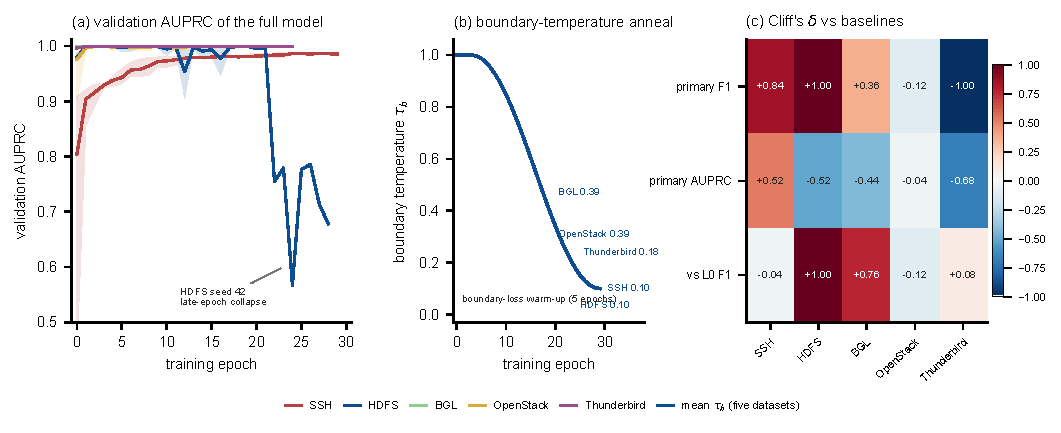
\includegraphics[width=\textwidth]{figures/SuppFig1_training_dynamics.pdf}
\caption*{\textbf{Supplementary Figure S1.} Training dynamics and paired effect sizes. (a) Validation AUPRC against the training epoch for the five datasets (five seeds; line = mean, band = range). (b) The boundary-temperature anneal recorded during training. (c) Cliff's $\delta$ of the paired comparisons against the strongest controlled baseline and against the flat GRU baseline. The HDFS seed that collapses after epoch 23 is visible in (a) and is why model selection relies on validation-based early stopping.}
\end{figure}

\begin{figure}[htbp]
\centering
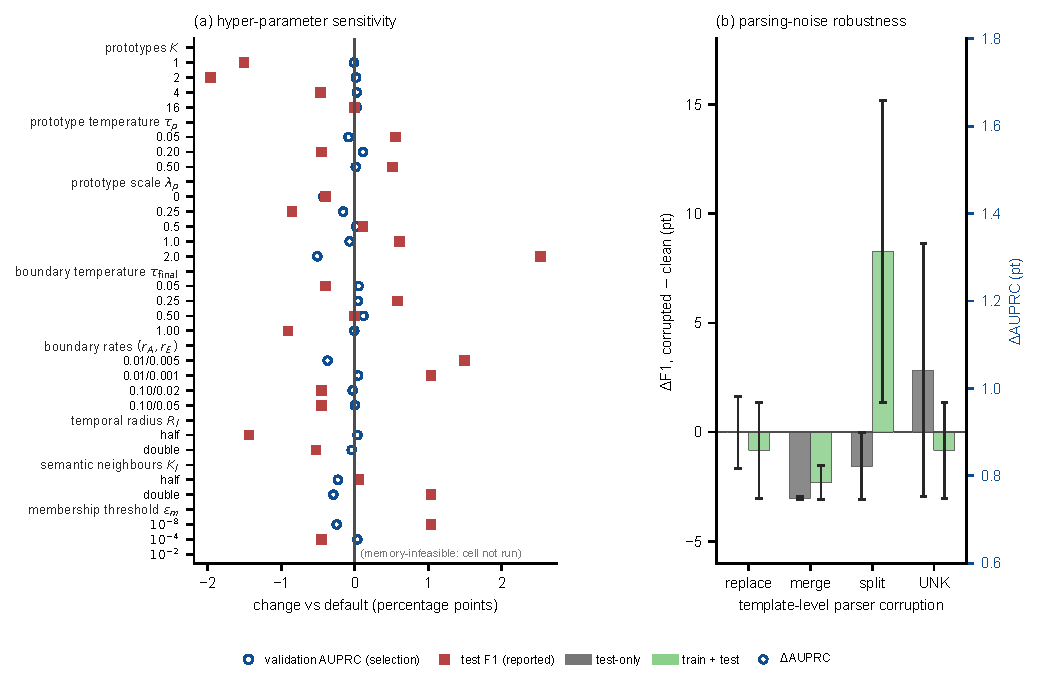
\includegraphics[width=\textwidth]{figures/SuppFig2_sensitivity_noise_robustness.pdf}
\caption*{\textbf{Supplementary Figure S2.} Hyper-parameter sensitivity and parsing-noise robustness. (a) Change of validation AUPRC (open circles, selection criterion) and test F1 (filled squares) relative to the default configuration, in percentage points. (b) Paired change under template-level parsing noise at a 20\% rewrite rate: bars are $\Delta$F1 (mean, range over two seeds) and open circles are $\Delta$AUPRC. Ranking quality is unchanged while F1 moves in both directions, i.e. the F1 movement reflects threshold calibration rather than a loss of detection ability.}
\end{figure}

\clearpage
\subsection*{Supplementary References}
\begin{enumerate}[label={\arabic*.},leftmargin=1.6em,itemsep=1pt]
\item Guo H, Yuan S, Wu X. LogBERT: log anomaly detection via BERT. In: 2021
International Joint Conference on Neural Networks (IJCNN), 2021.
\item Du M, Li F, Zheng G, Srikumar V. DeepLog: anomaly detection and diagnosis from
system logs through deep learning. In: Proceedings of the ACM SIGSAC Conference on
Computer and Communications Security, 2017: 1285--1298.
\item Meng W, Liu Y, Zhu Y, et al. LogAnomaly: unsupervised detection of sequential and
quantitative anomalies in unstructured logs. In: Proceedings of the 28th International
Joint Conference on Artificial Intelligence, 2019: 4739--4745.
\item Huang S, Liu Y, Fung C, et al. HitAnomaly: hierarchical transformers for anomaly
detection in system log. IEEE Transactions on Network and Service Management, 2020,
17(4): 2064--2076.
\item Lee Y, Kim J, Kang P. LAnoBERT: system log anomaly detection based on BERT masked
language model. Applied Soft Computing, 2023, 146: 110689.
\item Zhang C, Peng X, Sha C, et al. DeepTraLog: trace-log combined microservice anomaly
detection through graph-based deep learning. In: Proceedings of the 44th International
Conference on Software Engineering (ICSE), 2022: 623--634.
\item Liu F, Wen Y, Zhang D, et al. Log2vec: a heterogeneous graph embedding based
approach for detecting cyber threats within enterprise. In: Proceedings of the ACM SIGSAC
Conference on Computer and Communications Security, 2019: 1777--1794.
\item Ailabouni F, Rom\'an-Gallego J \'A, P\'erez-Delgado M L, Grande P\'erez L.
Boundary-aware contrastive learning for log anomaly detection. Applied Sciences, 2026,
16(7): 3208.
\item van Ede T, Aghakhani H, Spahn N, et al. DeepCASE: semi-supervised contextual
analysis of security events. In: Proceedings of the IEEE Symposium on Security and
Privacy, 2022: 522--539.
\item Hou Z, Ghashami M, Kuznetsov M, Torkamani M. HLogformer: a hierarchical transformer
for representing log data. arXiv preprint arXiv:2408.16803, 2024.
\item He P, Zhu J, Zheng Z, Lyu M R. Drain: an online log parsing approach with fixed
depth tree. In: Proceedings of the IEEE International Conference on Web Services (ICWS),
2017: 33--40.
\end{enumerate}

\end{document}
